\documentclass{sig-alternate-05-2015}

\usepackage{graphicx}
\usepackage{url}
\usepackage{enumitem}
\usepackage{caption}
\usepackage{listings}
\usepackage{textcomp}

\lstset{basicstyle=\ttfamily, captionpos=b}
\usepackage{xcolor}
\newcommand\todo[1]{\textbf{\textcolor{red}{#1}}}
\newcommand{\lstul}[1]{\underline{\mbox{\tt #1}}}

\toappear{}
\begin{document}

% Copyright
\setcopyright{acmcopyright}
%\setcopyright{acmlicensed}
%\setcopyright{rightsretained}
%\setcopyright{usgov}
%\setcopyright{usgovmixed}
%\setcopyright{cagov}
%\setcopyright{cagovmixed}


% DOI
\doi{10.475/123_4}

% ISBN
\isbn{123-4567-24-567/08/06}

%Conference
\conferenceinfo{PLDI '13}{June 16--19, 2013, Seattle, WA, USA}

\acmPrice{\$15.00}

%
% --- Author Metadata here ---
\conferenceinfo{WOODSTOCK}{'97 El Paso, Texas USA}
%\CopyrightYear{2007} % Allows default copyright year (20XX) to be over-ridden - IF NEED BE.
%\crdata{0-12345-67-8/90/01}  % Allows default copyright data (0-89791-88-6/97/05) to be over-ridden - IF NEED BE.
% --- End of Author Metadata ---

\title{Automatic Trigger Generation for Rule-based Smart Homes}
%
% You need the command \numberofauthors to handle the 'placement
% and alignment' of the authors beneath the title.
%
% For aesthetic reasons, we recommend 'three authors at a time'
% i.e. three 'name/affiliation blocks' be placed beneath the title.
%
% NOTE: You are NOT restricted in how many 'rows' of
% "name/affiliations" may appear. We just ask that you restrict
% the number of 'columns' to three.
%
% Because of the available 'opening page real-estate'
% we ask you to refrain from putting more than six authors
% (two rows with three columns) beneath the article title.
% More than six makes the first-page appear very cluttered indeed.
%
% Use the \alignauthor commands to handle the names
% and affiliations for an 'aesthetic maximum' of six authors.
% Add names, affiliations, addresses for
% the seventh etc. author(s) as the argument for the
% \additionalauthors command.
% These 'additional authors' will be output/set for you
% without further effort on your part as the last section in
% the body of your article BEFORE References or any Appendices.

\numberofauthors{2} %  in this sample file, there are a *total*
% of EIGHT authors. SIX appear on the 'first-page' (for formatting
% reasons) and the remaining two appear in the \additionalauthors section.
%
\author{
% 1st. author
\alignauthor
Chandrakana Nandi\\
       \affaddr{University of Washington, Seattle}\\
       \email{cnandi@cs.washington.edu}
\alignauthor Michael D. Ernst\\
       \affaddr{University of Washington, Seattle}\\
       \email{mernst@cs.washington.edu}
%Anonymous submission
}

\maketitle
\begin{abstract}
Trigger action programming is one of the most commonly used programming models for end user customizable smart homes~\cite{practical-tap} that allows them to write their own automation rules. Despite of that, recent studies have shown that end users often write incorrect rules and have difficulty in interpreting their behavior correctly~\cite{Huang}. In this paper, we propose a technique to prevent users from making a certain type of mistake in the rules--\textit{errors due to too few triggers}. We found that due to fewer firings of a rule, even a correctly written \textit{action} can lead to security vulnerabilities and unexpected behavior in a smart home. Our solution automatically generates trigger conditions based on the actions written by the end user by performing a static analysis of the actions and extracting potential triggers. It can also identify missing triggers if some of the triggers are already written by the users. We have developed our tool and tested it on 116 end-user written rules based on one of the most popular open source home automation frameworks called openHAB. By manual inspection of the suggested triggers, we found that 73\% of the rules had fewer number of triggers than required for their correct behavior. 
\end{abstract}

\printccsdesc


\keywords{Security, Home automation, Trigger action programming, Static analysis}

\section{Introduction}
Most home automation platforms have a major end-user component: they decide what actions should be taken by what device under what conditions~\cite{Newmannowwere}. For example, Samsung SmartThings~\cite{samsung} allows the users to create their own automation rules through their ``SmartApps" feature, while Apple HomeKit~\cite{homekit} allows the users to set up additional conditions to govern when an action should take place. A recent study~\cite{practical-tap} has shown that rule-based systems are one of the most practical solutions for enabling end-users to customize the behavior of their smart homes. A rule-based language has two main components: actions to be executed when a rules fires and triggers that cause a rule to be fired. This is also called Trigger Action Programming (TAP). Listing~\ref{lst:rule} shows the syntax of a rule. The part between \texttt{when} and \texttt{then} is the trigger block and the part between \texttt{then} and \texttt{end} is the action block. There can be multiple triggers in the trigger part. A rule engine is responsible for firing of the rules when the triggers are satisfied.
\begin{lstlisting}[caption={Syntax of rules.},label={lst:rule}]
rule "Rule name"
when
  <trigger_condition_1> OR
  <trigger_condition_2> OR 
  ...	
then
  <action_block>
end
\end{lstlisting}
Some other recent studies~\cite{Huang},\cite{wild-tap} have shown that even though TAP is the most commonly used and practical approach for home automation, end users often have difficulty in correctly interpreting the outcome of TAP and make errors in writing trigger-action programs with the desired behavior. These errors could be in 1) writing the actions, or 2) writing the triggers or 3) both. In a heterogeneous system like a smart home where there are multiple interacting devices, it is common for the rules to interact. As a result, an error in one rule can propagate to others and cause unexpected behavior or security vulnerabilities in different parts of the house. In this paper, we propose a solution to make it easier for the end users to write home automation rules correctly. Our approach eliminates one category of errors in the rules--errors due to too few triggers. By doing a static analysis of the actions, we automatically generate the trigger conditions so that the user does not have to worry about including the \textit{correct} and \textit{sufficient number} of trigger conditions in the rules. Our approach can identify potential bugs in the rules statically and thus ensure that the rules are free from \textit{errors due to too few triggers} once they are deployed. To the best of our knowledge, there has not been any prior research on analysing end-user written rules for home automation.

We analysed 116 home automation rules written by end users in the openHAB framework~\cite{openhab} and implemented our tool for rules written in the domain specific languages provided by openHAB, but our idea can be used for any rule-based system.
openHAB is an open source home automation framework which supports 135 technologies, including more than 50 devices, cloud services like Twitter, DropBox, Google Calendar etc. and multiple communication protocols~\cite{openhabtech}. It has UI support for Android and iOS and an IFTTT integration~\cite{ifttt}. It is a java based solution which can be run on standard Linux, Windows and MacOS X machines as well as on embedded platforms such as Raspberry Pi and Cubietruck. We chose to work with openHAB because
1) it is open source and that allowed us to access their code base and understand its functioning 2) it supports many devices and technologies and has about 50,000 downloads in the Google Play store with a rating of 4.4/5 and 3) unlike most proprietary solutions, openHAB does not require any hardware installation and is completely technology and vendor agnostic, which makes it more accessible to home owners. 

By a combination of static analysis and manual inspection of the results of the analysis, we found 73\% rules to be vulnerable and deviating from the expected behavior due to lack of trigger conditions. Our results indicate that for all rule-based smart home solutions, together with strong security guarantees provided by home automation framework developers, there is a serious need to focus on the end-user written rules because these are mostly written by non-programmers and are often prone to errors. 
Our contributions are the following:
\begin{enumerate}[topsep=0pt,itemsep=-1ex]
\item Analysis of end-user written rules for home automation and identifying and defining the problem of \textit{too few triggers}.
\item  Designing and implementing a static analysis tool that can 
\begin{itemize}[topsep=-10pt,itemsep=-1ex,partopsep=1ex,parsep=1ex]
\item suggest event-based triggers based on the actions written by end-users.
\item identify missing triggers 
\end{itemize}
\item Evaluating our tool on real end-user written rules for home automation in the openHAB framework.
\end{enumerate}

\section{Motivating Example}
\label{sec:motivation}
Consider the rule in listing~\ref{lst:away} which is written by an end user using the OpenHAB smart home framework. The name of the rule is \texttt{Away rule}. An \texttt{Item} represents the states of a device in the house. They can be read from or written to in order to interact with the devices. The state of an item can be changed by the end user through the UI of the openHAB application on a smart phone or on a desktop installation.
\begin{lstlisting}[caption={Rule for setting the Away or Sleeping state.},label={lst:away}]
rule "Away rule"
when
  Item State_Away changed 	
then
  if(State_Away.state == ON){
    if(State_Sleeping.state != OFF){
      postUpdate(State_Sleeping,OFF)
    }
  }
end
\end{lstlisting}
This rule is supposed to set the value of \texttt{State\_Away} to \texttt{ON} when everyone is away. It also sets \texttt{State\_Sleeping} to \texttt{OFF} if it currently \texttt{ON} so that both \texttt{State\_Away} and \texttt{State\_Sleeping} are not \texttt{ON} simultaneously. However, the trigger for this rule only contains \texttt{State\_Away}. As a result, this rule is only fired when \texttt{State\_Away} is changed by the end user. However, if the value of \texttt{State\_Sleeping} is changed after the value of \texttt{State\_Away}, then the rule is not fired due to which, it allows both values to be set at the same time. This deviates from the expected behavior of the rule--it is no longer clear whether the home inhabitants are away or inside sleeping. This is also a security vulnerability because if this rule triggers another rule for turning on the security alarm in the house and the security alarm is meant to be off when people are at home but on when they are away, then it could get wrongly deactivated if the value of \texttt{STATE\_SLEEPING} is set to \texttt{ON}. Figure~\ref{fig:awayrule} shows a snapshot of the desktop application with both states being set to \texttt{ON}. 
\begin{figure}
\centering
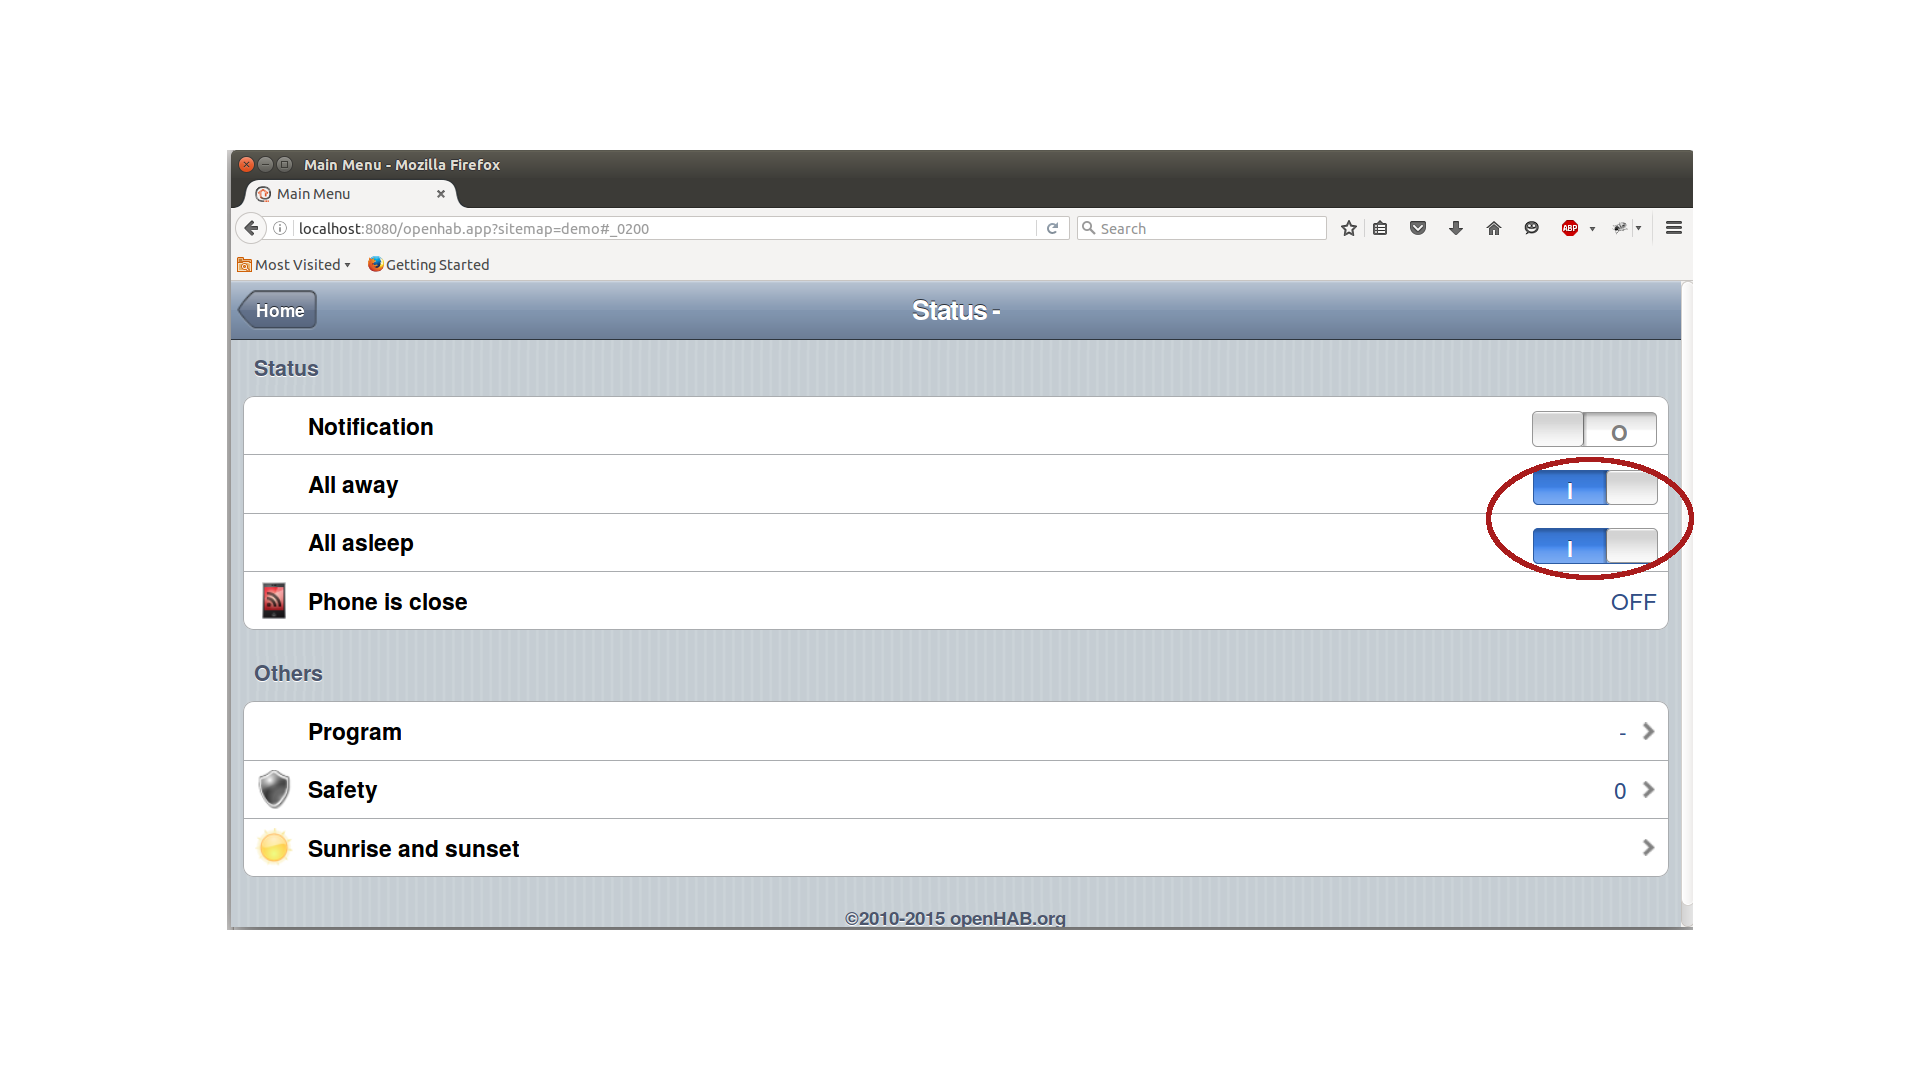
\includegraphics [trim=1cm 13cm 0 0, scale=0.14]{images/openhab-runtime.png}
\caption{Desktop UI showing that it is possible to set both \texttt{State\_Away} and \texttt{State\_Sleeping} to \texttt{ON} at the same time. Blue indicate that they are \texttt{ON}.}
\label{fig:awayrule}
\end{figure}
This example shows that even if the action block of a rule is implemented correctly, not having all the correct triggers can lead to too few firings of the rule and thus, unexpected behavior. To solve this problem, we propose a technique based on static analysis that can automatically generate event-based triggers and also detect missing ones by analysing code in the action block. 
\begin{lstlisting}[caption={List of suggested and missing triggers shown by our tool for the Away rule.},label={lst:output}]
rule:Away rule
suggested trigger: State_Away
suggested trigger: State_Sleeping
------------------------------
rule:Away rule
missing trigger: State_Sleeping
\end{lstlisting}
The result of running our tool on the rule in listing~\ref{lst:away} is shown in listing~\ref{lst:output}. It shows two features of the tool: suggesting all event based triggers and identifying missing triggers when some triggers are already written by the end user.

\section{Threat model}
Our focus is on security vulnerabilities that result due to incorrectly written automation rules by the home inhabitants or by an adversary although the former is more likely. 
We target one category of errors in the rules: \textit{errors due to too few triggers}. Our approach can prevent any attack that relies on incorrect number of rule firings. One such example is described in section~\ref{sec:motivation}.

We assume that the action block of the rules is written correctly and rely on it for generating the trigger conditions.

We trust that the devices in the house are not compromised and once they receive a command, they execute it. We also trust the rule engine and the home automation OS for which the rules are written.

\section{\MakeLowercase{open}HAB background}
openHAB~\cite{openhab} is an open source software for integrating different types of smart technologies in a home. openHAB has a runtime implemented in Java and a designer which is used by end users for configuring the homes. 

The runtime provides a communication platform between the devices. There are currently about 135 devices, protocols and cloud technologies supported by openHAB. These are connected by means of an event bus. Figure~\ref{fig:framework} shows the main components of the openHAB framework. The item repository stores the states of the devices. It is connected to the UI and the rule base. Changes to the states can be made through the UI and by rule firings. The latest state is communicated to the actual device through the event bus. The bindings are libraries that connect the physical devices to the openHAB framework. As shown in the figure, there are two types of events that are communicated by the event bus--1) commands: causing an action or change of state in a device, such as \texttt{ON}, \texttt{OFF}, \texttt{UP}, \texttt{DOWN} and 2) updates: informing the UI component or the rule engine or other devices about a change in the state of a device.
\begin{figure}
\centering
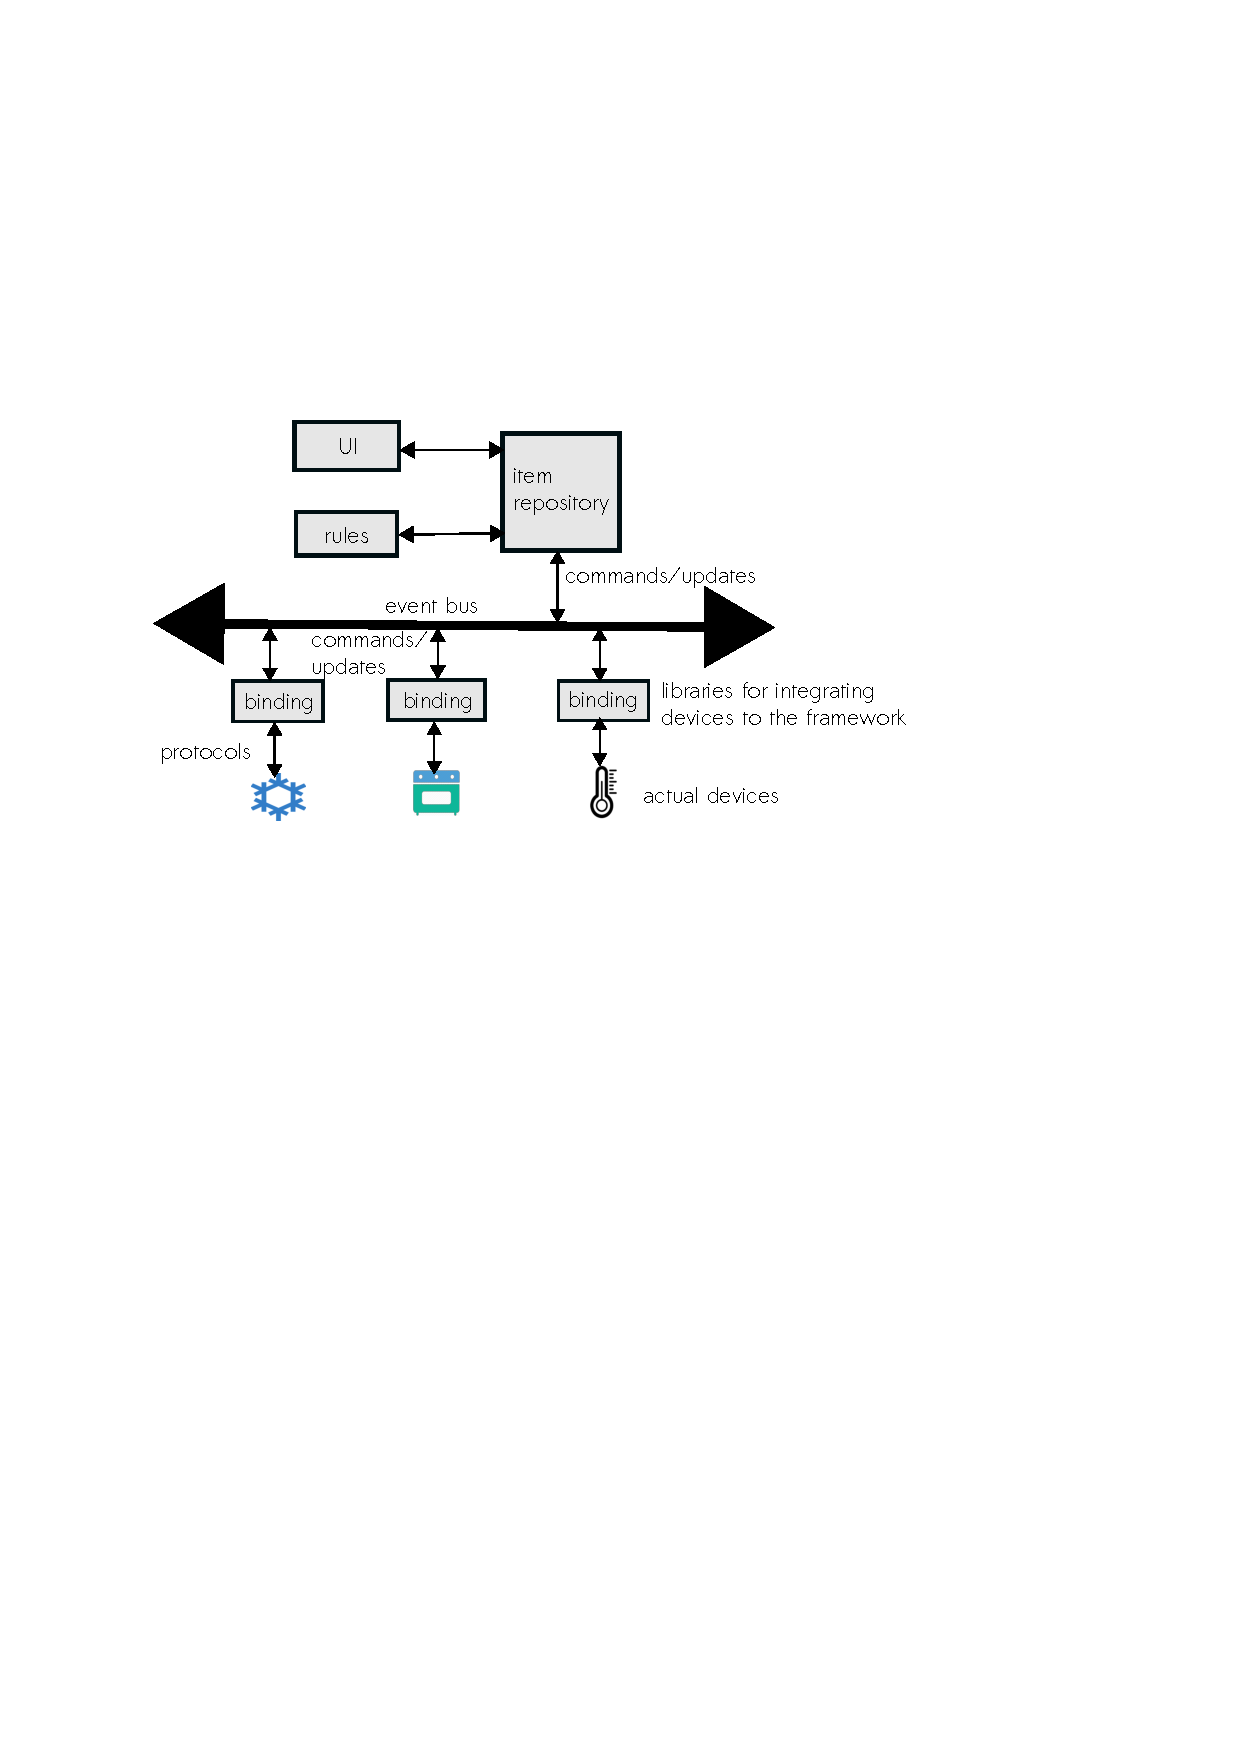
\includegraphics [trim=-2cm 15cm 0 6.5cm, scale=0.4]{images/framework.pdf}
\caption{openHAB framework.}
\label{fig:framework}
\end{figure} 

The designer includes an IDE for writing the configuration files to customize the home. The main configuration files include a \textit{.rules} file containing the automation rules, a \textit{.items} file (storing the states of the devices installed) and a \textit{.sitemap} file that maps items to elements in the UI. Each of these are written in small domain specific languages developed using the xtext framework~\cite{xtext}. The action block in the rules, also called the \textit{script} is written in a Java like language called xbase, which is implemented using xtext. For our research, we required access to the item files and the rule files. 
\subsection{Items}
The item file lists the states of all the devices in the house that are to be included in the automation. Every item has a type that indicates the values it can store and the commands it can receive. Items can also be grouped together--all lights in the living room can be in one group so that they can be controlled together. There are 11 types of items that are currently supported. Listing~\ref{lst:items} shows the syntax of an item definition (contents in [~] are optional) and two entries in a sample item file. The binding part is responsible for connecting the item to an actual device ID.
\begin{lstlisting}[caption={Syntax and two examples of item definitions.},label={lst:items}]
<type> <name> ["label"] [<icon>] 
              [(group*)] [{binding}]
Switch DemoSwitch  "Switch"
Contact Window_Bedroom "Bedroom" 
        (Bedroom, Windows)
\end{lstlisting}
 
\subsection{Rules}
Listing~\ref{lst:rule} shows the syntax of the rules. There are three types of triggers.
\begin{enumerate} [topsep=0pt,itemsep=-1ex]
\item event-based triggers: These triggers are related to changes in the state of a device. Some examples--\\
\texttt{Item LightSwitch received command} \\
\texttt{Item State\_Away changed}
\item temporal triggers: They cause actions to happen at a certain time. An example--\\ \texttt{Time cron "second minute hour day month weekday year"}
\item system triggers: There are two system triggers--system start up and system shut down.
\end{enumerate}
\subsection{Actions}
\label{subsec:actions}
Actions are predefined methods in Java that can be used in the scripts of the rules. The openHAB runtime provides a core set of actions but more can be implemented for specific devices by the respective manufacturers. The most important core actions for the purpose of our analysis are the event bus actions: \texttt{sendCommand(String itemName, String commandName)}, \texttt{postUpdate(String itemName, String stateValue)}. The entire list of actions can be found in the openHAB wiki~\cite{openhabwiki}.

\section{Errors due to too few triggers}
\emph{Problem Definition}. Errors due to too few triggers is a condition where an insufficient number of triggers leads to fewer firing of a rule thereby leading to unexpected behavior or security vulnerabilities. \\

\emph{Goal}. Our goal is to prevent end users from making errors due to too few triggers--we want to ensure that all the correct triggers are included in the rules. \\

\emph{Approach}. Our approach is to automatically generate all the correct trigger conditions from the actions written by the end users. We developed a static technique to achieve this so that the rules do not need to be fired at all until all the correct triggers are included. Figure~\ref{fig:design} shows the design of our tool. It takes as input a \textit{rules} file and and \textit{items} file. The technique is explained below.
\begin{enumerate}
\item By statically analysing the AST of the script, $S$, we first identify all the items that appear in a rule, $R$. This is an exhaustive list of all potential event-based triggers. Let this list be $T$.
\item Naively adding all $t \in T$ as triggers of $R$ would either unnecessarily fire $R$ too many time or add redundant triggers which would make $R$ unnecessarily complicated. Hence, we apply an elimination technique to get rid of triggers that are not relevant. The following definitions are used in the elimination algorithm. 

\emph{Live item}. An item is live in R if its value is read before it is written to in the rule script. 

\emph{Dependent item}. We define an item to be \emph{dependent} in $R$ if its value is computed based on other items or variables in the rule--this implies that the item is \emph{not live}. 
 
\emph{Independent item}. We define an item to be \emph{independent} in $R$ if  its value is directly obtained from a sensor or a user's input and not computed based on any other item or variable--this implies that the item is \emph{live} in $R$. 

\emph{Redundant trigger}. We define an event-based trigger to be redundant if inclusion of the trigger in a rule \emph{never} changes the state of any item or the value of any variable involved in the rule when the rule is fired due to it.
\begin{enumerate}
\item  An item $d$ which is not \textit{live} in $R$ is not included in $T$ because it is redundant. As a corollary, if $d$ is dependent, it is also not included it $T$.\\
\emph{Theorem}. If $d$ is not live in $R$, then it is a redundant trigger.\\
\emph{Proof}. Let us assume that $d$ is not redundant. That means it must change the value of some item or variable in $R$ in some firing. Let this item or variable be $a$. Since $d$ is not live, its value is never read before it is written to. The following cases are possible:
\begin{itemize} [topsep=-2pt, itemsep=-1pt]
\item $d$ is assigned a constant value. In this case, $d$ as a trigger does not change the value of $a$ because $d$'s value is always the same (as long as the script of R  itself is not changed).
\item $d$ is some function of other items, $i_1, i_2, ..., i_n$ and variables $v_1, v_2, ..., v_m$ in $R$. In this case, $d$ as a trigger will still not affect the value of $a$ because $d$'s own value depends on the values of items $i_1, i_2, ..., i_n$--adding the live items from $i_1, i_2, ..., i_n$ as triggers would be sufficient.
\end{itemize}
\end{enumerate}
\end{enumerate}

\emph{Scope}. The algorithm for automatically generating triggers described above targets event-based triggers only--our tool does not aim to suggest temporal or system triggers. This is because temporal and system based triggers are highly dependent on the end user's preference and without any additional annotations from the user, it is impossible to suggest a generic temporal or system trigger that will be applicable to all users. Since our tool does not require any annotations from the end user, the scope of our tool is limited to event-based triggers. This means that if the end user intends a rule to be fired only under system or temporal triggers, the suggestions provided by our tool will not be useful. Table~\ref{tab:scope1} summarizes the usefulness of our tool for suggesting triggers with respect to the conditions under which the user actually expects the rule to be fired.
\begin{table}[h]
\centering
\begin{tabular}{|l|l|}
\hline
user's expectation & usefulness \\ \hline
event-based & high \\ \hline
combination of event-based, temporal, system  & medium \\ \hline
temporal & low \\\hline
system & low \\ \hline
combination of temporal, system & low  \\ \hline

\end{tabular}
\caption{Scope of our tool for suggesting triggers only based on the rule script (no triggers written by the user). High indicates that all the suggestions are useful, medium indicates that only the event-based suggestions are useful and none indicates that none of the suggestions are useful. }
\label{tab:scope1}
\end{table}

As mentioned before, our tool can also identify triggers that are missing, in case the end user already has written some triggers. Table~\ref{tab:scope2} summarizes the scope of our tool for identifying missing triggers. If the triggers written by the end users only include system and temporal triggers, then our tool does not suggest any other event-based trigger because that would modify the behavior of the rule. If however, at least one event-based trigger is included, then our tool identifies all other event-based triggers that should also be included. 
 
\begin{table}[h]
\centering
\begin{tabular}{|l|l|}
\hline
user written triggers & tool's output \\ \hline
at least one event-based & missing event-based triggers \\ \hline
only temporal & none \\\hline
only system & none \\ \hline
temporal and system & none  \\ \hline
\end{tabular}
\caption{Scope of our tool for detecting missing triggers when some triggers are already written by the user.}
\label{tab:scope2}
\end{table}

\begin{figure*}
\centering
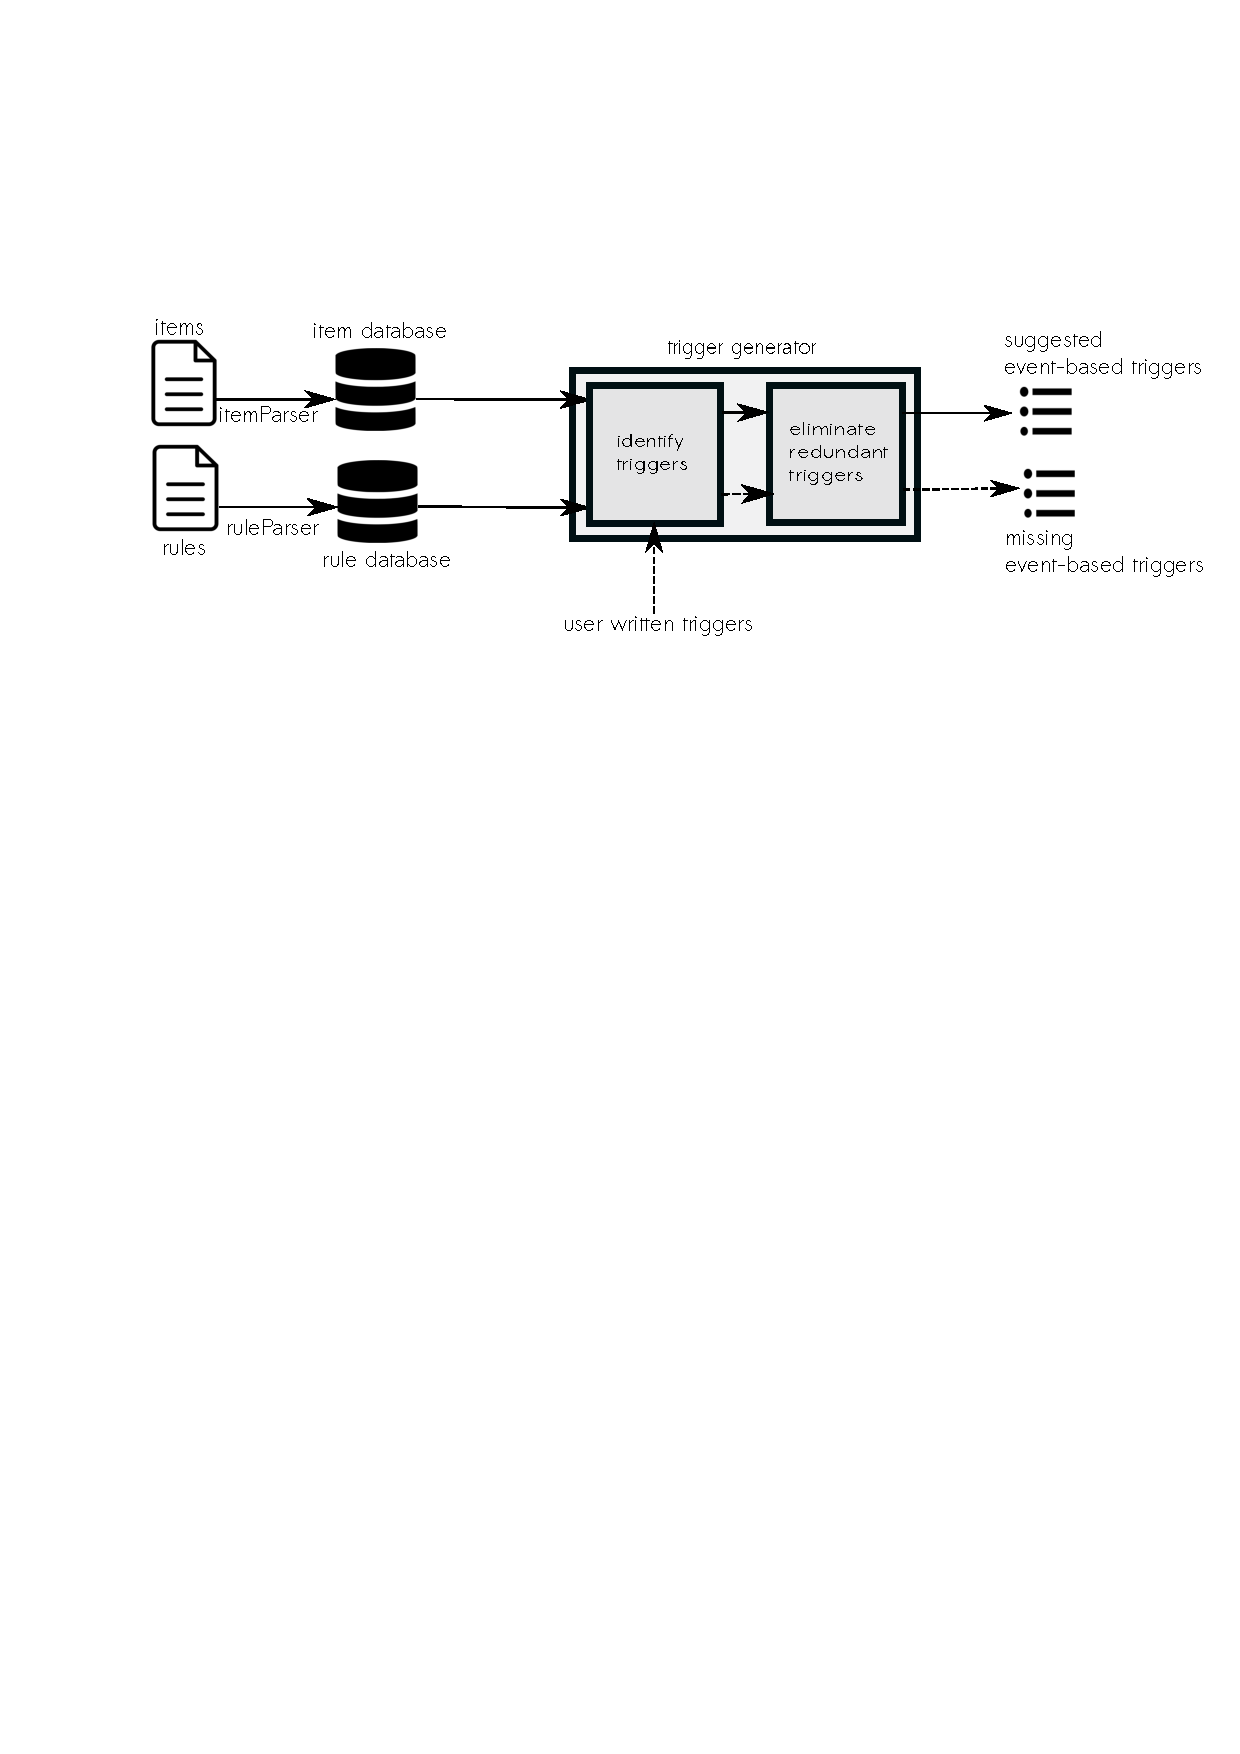
\includegraphics [trim=0cm 18cm 0 5cm, scale=0.8]{images/design.pdf}
\caption{Design of trigger generator tool.}
\label{fig:design}
\end{figure*} 

\section{Implementation}
We implemented the automatic trigger generator and missing trigger identifier in Java. It involved $\sim$ 3000 LOC. Our tool can be used directly on a rule file without any pre-processing of the rules. 

We used the AST generated by xtext for the rule \textit{scripts} and visited the nodes in the tree to extract relevant information such as the names of the device states used in the method calls or in conditional statements. 
\todo{[do people care to know about the details?]}
 
\section{Experimental Evaluation}
We evaluated our tool on 116 end user written rules. We obtained the rules from links provided on the openHAB wiki~\cite{data1},\cite{data2}. It took $\sim$ 7.12 ms for the tool to generate the triggers and find the missing triggers for all the rules. Tables~\ref{tab:results1} and ~\ref{tab:results2} show the summary of our results. For 99 out of the 116 rules, our tool suggested a list of all correct triggers and for 74 out the 116 rules, our tool found missing triggers when some triggers were already provide by the users.  
\begin{table}[h]
\centering
\begin{tabular}{|c|p{1.1cm}|}
\hline
\# suggested triggers & \# rules \\ \hline
0 & 17\\ \hline
1 & 17\\ \hline
2 & 40\\ \hline
3 & 18\\ \hline
4 & 8\\ \hline
5 & 8\\ \hline
6 & 4\\ \hline
8 & 1\\ \hline
9 & 1\\ \hline
10 & 1\\ \hline
18 & 1\\ \hline
\end{tabular}
\caption{Summary of results for suggested trigger.}
\label{tab:results1}
\end{table}

\begin{table}[h]
\centering
\begin{tabular}{|c|p{1.1cm}|}
\hline
\# missing triggers & \# rules \\ \hline
0 & 42 \\\hline
1 & 54 \\\hline
2 & 3 \\\hline
3 & 5\\\hline
4 & 7\\\hline
5 & 2\\\hline
8 & 1 \\\hline
9 & 1 \\\hline
14 & 1 \\\hline
\end{tabular}
\caption{Summary of results for missing triggers.}
\label{tab:results2}
\end{table}

\section{Related work}
\todo{\cite{smartthings16, todayToTomorrow, rvs, homer, utea}
Recent work has mentioned possible security loopholes in smart homes~\cite{yoshi, dhanjani, jung}. there is more, need to add from previous documents I wrote.}

\section{Conclusions}
End users have a major role in home automation--they decide the automation rules for the devices. Not surprisingly, our research shows that these end user written rules \textit{are} a major source of security vulnerability in smart homes.
We observed that a common error made by end users while writing the rules is having insufficient number of triggers, leading to fewer firings of the rules than necessary. To prevent this problem, we developed a tool that can automatically generate trigger conditions based on the actions in a rule as well as identify missing triggers if some of them are already provided. This reduces the burden of end user by assisting them in including all the required triggers. 

We evaluated our tool on real home automation rules written by end users and found that out of 116 rules, 74 had insufficient number of triggers. By manual inspecting the suggestions provided by the tool, we found that each one of them were relevant and including them in the rules prevented the unexpected behaviors observed previously. 


\section{Acknowledgements}
We thank Franziska Roesner for her valuable feedback and Jeanette Daum for contributing to an earlier version of this project.
\bibliographystyle{abbrv}
\bibliography{sigproc}  

\end{document}
